\documentclass[11pt, oneside]{article}   	% use "amsart" instead of "article" for AMSLaTeX format
\usepackage{geometry}                		% See geometry.pdf to learn the layout options. There are lots.
\geometry{letterpaper}                   		% ... or a4paper or a5paper or ... 
%\geometry{landscape}                		% Activate for rotated page geometry
\usepackage[parfill]{parskip}    			% Activate to begin paragraphs with an empty line rather than an indent
\usepackage{graphicx}				% Use pdf, png, jpg, or eps§ with pdflatex; use eps in DVI mode
								% TeX will automatically convert eps --1 pdf in pdflatex		
\usepackage{bbm}
\usepackage{amssymb,amsmath,amsthm,bm,pgfplots,tikz}
\usepackage{mathtools}
\usepackage{enumitem}
\usepackage{comment}
\usepackage{pgfplots}
\usepackage[utf8]{inputenc}
\usepackage{xeCJK}
\setCJKmainfont{NotoSansCJKtc-Regular.otf}



\usetikzlibrary{arrows}

\def\firstcircle{(90:1.75cm) circle (2.5cm)}
\def\secondcircle{(210:1.75cm) circle (2.5cm)}
\def\thirdcircle{(330:1.75cm) circle (2.5cm)}


\definecolor{pointcolor}{RGB}{203, 67, 53}

\newcommand{\E}[1]{\mathbb{E}\left[#1\right]}

\renewcommand{\qedsymbol}{}



\newenvironment{Solution}[1][Sol]{%
  \begin{proof}[#1]$ $\par\nobreak\ignorespaces
	\qquad
}{%
  \end{proof}
}

\title{Data Science and Social Inquiry: HW2}
\author{R11323006 陳柏語 R11323015 張藝懷 B07303119 劉怡廷
\\B08303124 劉詠晴 B09303052 蔡尚恩
}
						

\begin{document}

\maketitle


% Type your answer inside the Solution block.

\section*{Question 1: PCA with non-diagonal covariance matrix}

\begin{enumerate}[label = (\emph{\alph*})]
	\item (2 pts) What is the first principal component? 
	Explain how you reach your answer carefully and write down its coefficients.
	\begin{Solution}
		%Your answer should be some linear combinations of the 5 variables
		
		$\mathop{max}_{\limits{b_1\in \mathbb{R}^P}}{b_1}'D{b_1}$ s.t.${b_1}'b_1=1$\\
		$\mathop{max}_{\limits{b_1\in \mathbb{R}^P}}{b_1}'D{b_1}=0.855{b_{11}}^2+0.942{b_{12}}^2+0.738{b_{13}}^2+0.109{b_{14}}^2+2.024{b_{15}}^2$s.t.${b_1}'b_1=1$\\
		
		Since 2.024 is the biggest number in five coefficients, we can know $b_{15}=\pm1,b_{11}=b_{12}=b_{13}=b{14}=0$
		
		$b=\left[\begin{array}{ccccc}
		0 \\
		0\\
		0\\
		0\\
		1\\
		\end{array}\right]=P'a_{i}\\
		a=Pb=\left[\begin{array}{ccccc}
		-0.135 & -0.763 & 0.606 & -0.182 & 0.006\\
		-0.27 & -0.477 & -0.745 & -0.271 & 0.268\\
		-0.405 & -0.191 & -0.062 & 0.892 & -0.015\\
		-0.539 & 0.095 & -0.065 & -0.242 & -0.798\\
		-0.674 & 0.381 & 0.266 & -0.197 & 0.539\\
		\end{array}\right]\left[\begin{array}{ccccc}
		0 \\
		0\\
		0\\
		0\\
		1\\
		\end{array}\right]=\left[\begin{array}{ccccc}
		0.006\\
		0.268\\
		-0.015\\
		-0.798\\
		0.539\\
		\end{array}\right]$
		
		$PC_{1}= a'X =\left[\begin{array}{ccccc}
		0.006 & 0.268 & -0.015 & -0.798 & 0.539
		\end{array}\right]\left[\begin{array}{ccccc}
		X_{1} \\
		X_{2}\\
		X_{3}\\
		X_{4}\\
		X_{5}\\
		\end{array}\right]\\=0.006X_{1}+0.268X_{2}-0.015X_{3}-0.798X_{4}+0.539X_{5} $
		
		
		
		
	\end{Solution}


	\item (1 pt) Calculate the proportion of variance explained by each component
	and use them to make the scree plot. 
	\begin{Solution}
	
    $\sum_{i=1}{p}\lambda_{i} = 0.855+0.942+0.738+0.109+2.024 = 4.668\\\\
    \frac{2.024}{4.668}=0.4335904\\\\
    \frac{0.942}{4.668}=0.20179949\\\\
    \frac{0.855}{4.668}= 0.18316195\\\\
    \frac{0.738}{4.668}=0.15809769\\\\
    \frac{0.109}{4.668}=0.02335047$



			\begin{center}
				\begin{tikzpicture}[scale=0.8]
					\begin{axis}[
						xlabel = Component Number,
						ylabel = Eigenvalue,
						x post scale = {1.5},
						xtick = {1,...,5},
					]
						\addplot[pointcolor, mark=*] table[header = false]
						{
							1 0.4335904
							2 0.20179949
							3 0.18316195
							4 0.15809769
							5 0.02335047
						};
					\end{axis}
				\end{tikzpicture}
			\end{center}
	\end{Solution}
				
\end{enumerate}





\section*{Question 2: Prototyping CEO's behavior}

\begin{enumerate}[resume*] 
	\item (1 pt) Every data analysis should start with examining the raw data.
			     Use a box plot to summarize the seven marginal distributions.
	\begin{Solution}
		% Hint: You might need to groupby id first.
		%\includegraphics[scale=0.6]{}
        \includegraphics[scale=0.4]{c.png}\\
	\end{Solution}
	\item (1 pt) Use a heatmap to summarize the correlations between the number of activities.
				 Which type correlates with type \textbf{politicians} most?
	\begin{Solution}
		%\includegraphics[scale=0.8]{...}
		\begin{center}
		\includegraphics[scale=0.6]{d.png}\\
		\end{center}
		We can observe that type govoff correlates with type politicians most.
	\end{Solution}
	

	\item (1 pt) Run PCA. What is the first principal component?
	\begin{Solution}
		$PCA_{1}= 0.954X_{1}+0.252X_{2}+0.002X_{3} +0.013X_{4}-0.003X_{5}+0.109X_{6}
  +0.115X_{7}$
	\end{Solution}
	\item (1 pt) Make the scree plot. How many principal components are needed to explain 70\% of the variation?
	\begin{Solution}

\textbf{Scree Plot}\\
			\begin{center}
				\begin{tikzpicture}[scale=0.8]
					\begin{axis}[
						xlabel = Component Number,
						ylabel = Eigenvalue,
						x post scale = {1.5},
						xtick = {1,...,7},
					]     
					
						\addplot[pointcolor, mark=*] table[header = false]
						{
							1 0.48063181
							2 0.25137937
							3 0.11362934
							4 0.05646524
							5 0.04252094
							6 0.03621477
							7 0.01915853
						};

					\end{axis}
				\end{tikzpicture}
			\end{center}\\
			
\textbf{Cummulative Explained Variance}\\
    \begin{center}
    \includegraphics[scale=0.8]{f.png}\\
    \end{center}
			Two principal components are needed to explain 70\% of the variation.
			
			
	\end{Solution}
	
	\item (1 pt) Put the first component on the x-axis and the second component on the y-axis.
				 Plot the coefficients of each variable. 
	 			 How would you interpret the first two components?

	\begin{Solution}
		% Replace 'your answer' by the coordinates of the projections onto PC1 and PC2.
	
     
			\begin{center}
				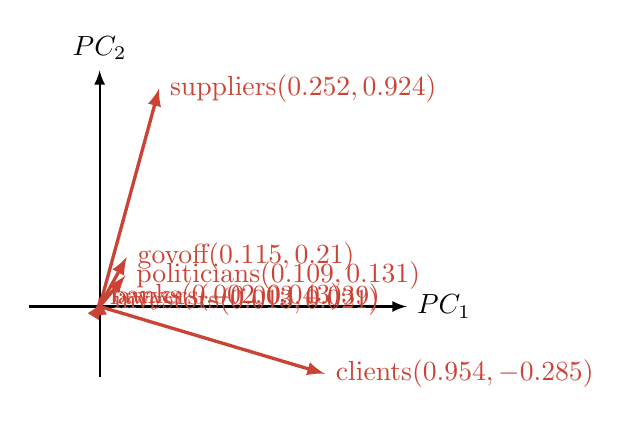
\begin{tikzpicture}[scale=3]
					\tikzstyle{component} = [-latex, pointcolor, very thick]
					
					\draw[-latex, thick] (-0.3,0) -- (1.3,0) node[right] {$PC_1$};
					\draw[-latex, thick] (0,-0.3) -- (0,1) node[above] {$PC_2$};
					



					\draw[component]   (0,0) -- (0.954,-0.285) node[right] {clients$(0.954,-0.285)$};
					\draw[component]   (0,0) -- (0.252,0.924) node[right] {suppliers$(0.252,0.924)$};
					\draw[component]   (0,0) -- (0.002,0.043) node[right] {banks$(0.002,0.043)$};
					\draw[component]   (0,0) -- (0.013, 0.021) node[right] {investors$(0.013,0.021)$};
					\draw[component]   (0,0) -- (-0.003, 0.039) node[right] {lawyers$(-0.003,0.039)$};
					\draw[component]   (0,0) -- (0.109, 0.131) node[right] {politicians$(0.109,0.131)$};
					\draw[component]   (0,0) -- (0.115, 0.21) node[right] {govoff$(0.115, 0.21)$};
				\end{tikzpicture}
			\end{center}\\
			
            $PC_{1}$ implies the strong relationship with the clients variable, since the coefficient is the highest.As for $PC_{2}$, it is the suppliers variable.
	\end{Solution} 
\end{enumerate}


\section*{Question 3: Practicing the hierarchical clustering algorithm}


\begin{enumerate}[resume*]
	\item (1 pt) Perform the hierarchical clustering with the average linkage. 
							Clearly indicate which observations are pooled in each step.
	\begin{Solution}

\textbf{STEP1}\\
		$distance_{1}=\left[\begin{array}{ccccc}
		0 & 3\sqrt{2} & \sqrt{10} & \sqrt{10} & \sqrt{10}\\
		3\sqrt{2} & 0 & 2\sqrt{10} & 2\sqrt{10} & 2\\
		\sqrt{10} & 2\sqrt{10} & 0 & 2 & 6 \\
		\sqrt{10}  & 2\sqrt{10} & 2 & 0 & 2\sqrt{10}\\
		\sqrt{10} & 2 & 6 & 2\sqrt{10} & 0\\
		\end{array}\right]$
		
		$ C_1:(X_1,Y_1)\\
		C_2:(X_2,Y_2),(X_5,Y_5)\\
		C_3:(X_3,Y_3),(X_4,Y_4)$
		
\textbf{STEP2}\\
		$distance_{2}=\left[\begin{array}{ccccc}
		0 & \frac{3\sqrt{2}+10}{2} & \sqrt{10}\\
		\frac{3\sqrt{2}+10}{2} & 0 & \frac{3\sqrt{10}+3}{2}\\
		\sqrt{10} & \frac{3\sqrt{10}+3}{2} & 0\\
		\end{array}\right]$
		
		$ C_1:(X_1,Y_1),(X_3,Y_3),(X_4,Y_4)\\C_2:(X_2,Y_2),(X_5,Y_5)$
		
		
\textbf{STEP3}\\
		$ C_1:(X_1,Y_1),(X_3,Y_3),(X_4,Y_4),(X_2,Y_2),(X_5,Y_5)$	
		
		
	
		
	\end{Solution}
	\item (1 pt) Perform the hierarchical clustering with the complete linkage.
	\begin{Solution}
	
\textbf{STEP1}\\
		$distance_{1}\left[\begin{array}{ccccc}
		0 & 3\sqrt{2} & \sqrt{10} & \sqrt{10} & \sqrt{10}\\
		3\sqrt{2} & 0 & 2\sqrt{10} & 2\sqrt{10} & 2\\
		\sqrt{10} & 2\sqrt{10} & 0 & 2 & 6 \\
		\sqrt{10}  & 2\sqrt{10} & 2 & 0 & 2\sqrt{10}\\
		\sqrt{10} & 2 & 6 & 2\sqrt{10} & 0\\
		\end{array}\right]$
		
		$ C_1:(X_1,Y_1)\\C_2:(X_2,Y_2),(X_5,Y_5)\\C_3:(X_3,Y_3), (X_4,Y_4)$
	
\textbf{STEP2}\\
		$distance_{2}\left[\begin{array}{ccccc}
		0 & 3\sqrt{2} & \sqrt{10}\\
		3\sqrt{2} & 0 & 2\sqrt{10}\\
		\sqrt{10} & 2\sqrt{10} & 0\\
		\end{array}\right]$
		
		$ C_1:(X_1,Y_1),(X_3,Y_3),(X_4,Y_4)\\C_2:(X_2,Y_2),(X_5,Y_5)$
		
\textbf{STEP3}\\
		$ C_1:(X_1,Y_1),(X_3,Y_3), (X_4,Y_4),(X_2,Y_2),(X_5,Y_5)$	
		
		
		
	\end{Solution}
\end{enumerate}


\end{document}  

